%Texlive-full Version 3.141592-1.40.3 (Web2C 7.5.6)
%Kile Version 2.0.83

\documentclass[a4paper,10pt]{article}
\usepackage[utf8]{inputenc}
\usepackage{graphicx}

\usepackage{lmodern}
\usepackage[a4paper]{geometry}

\usepackage{hyperref}

\usepackage{amsmath}
\usepackage{amssymb}
\usepackage{amsthm}

\usepackage{pstricks}
\usepackage{pst-node}
\usepackage{subfigure}
\usepackage[ddmmyyyy]{datetime} 
\newtheorem*{theorem*}{Theorem}
\newtheorem{theorem}{Theorem}
\newtheorem*{lemma*}{Lemma}
\newtheorem{lemma}{Lemma}
\newtheorem{proposition}{Proposition}
\newtheorem{corollary}[theorem]{Corollary}
\makeatletter
\renewcommand\theequation{\thesection.\arabic{equation}}
\@addtoreset{equation}{section}
\makeatother


\begin{document}
\begin{titlepage}
%%%%%%%%%%%%%%%%%%%%%%%%%%  LOGO  %%%%%%%%%%%%%%%%%%%%%%%%%%%%%%%%%%%%%%%%%
\begin{center}
\begin{pspicture}(-7,0)(7,2)
\rput(-8,1){\href{http://www.univ-paris-diderot.fr/english/sc/site.php?bc=accueil&np=accueil&g=m}{
\includegraphics[scale=1.2]{logo_p7}}}
\rput(4,2){\href{https://masterfinance.math.univ-paris-diderot.fr/}
	    {	\begin{tabular}{l}
		\resizebox{6cm}{2cm}{M2MO} \\
		\resizebox{6cm}{0.5cm}{DEA Laure Elie}  
		\end{tabular}
	    }
}

\rput(3,-0.5){
\begin{tabular}{l}
Prof.                                                    \\ 
\href{http://www.ann.jussieu.fr/~achdou/}{\textbf{ Yves Achdou} }          \\
\href{https://www.ljll.math.upmc.fr/~boka/}{\textbf{ Olivier Bokanowski}}   
\end{tabular}	    
}
%\psline(-7,0)(7,2)
\end{pspicture}
\end{center}



%%%%%%%%%%%%%%%%%% DOCUMENT TITLE %%%%%%%%%%%%%%%%%%%%%%%%%
\vspace{2cm}

\begin{center}
%\resizebox{14cm}{0.7cm}{High dimensional PDE solver for multi-asset pricing option}
\resizebox{14cm}{0.8cm}{Numerical Methods and PDE in Finance}
\end{center}
%%%%%%%%%%%%%%%%%% DOCUMENT TITLE %%%%%%%%%%%%%%%%%%%%%%%%%
\begin{center}
\huge{ Version : \today }
\end{center}


\begin{tabular}{l}
Students                                                                          \\ 
\href{mailto:chithanhnguyen.math@gmail.com}{\LARGE{\textbf{Chi Thanh NGUYEN}}}    \\
\href{mailto:nqcuong32@gmail.com}{\LARGE{\textbf{Quoc Cuong NGUYEN}}}
\end{tabular}



\vfill
\begin{abstract}
%\section*{Abstract}
Within the content of Master \href{https://masterfinance.math.univ-paris-diderot.fr/}{Random Modeling For Finance} program at University of Paris-Diderot Paris VII, we had a course about pricing financial option using numerical PDE method given by Mr \textbf{Y.Achdou} and Mr \textbf{O.Bokanowski}. We realized a project on resolving the multi-asset pricing option problem using Semi-Lagrangian PDE method. This project aims to initiate to the research of finance quantitative problems.  The whole project code is in C++ using the library ~\cite{BokanowskiLib} The references used in this project are ~\cite{Oksendal} , ~\cite{Bokanowski}, ~\cite{Achdou}. Our repport is organized as below. In the section 1, we present the Black-Scholes's model for a basket option, the transformation to a PDE's problem and a possible exact solution. In the section 2, we explain how we work with the discretization. Section 3 analyze the error of the discrete problem.
\end{abstract}
\end{titlepage}



\section{Basket Option Model}
The main task is to determine the price of a basket option with constant volatility. We consider a portfolio of $d$ assets with $\alpha_i$ quantities of underlying asset $S^i$. The problem is to determine the option price at all time $t$ given a payoff function $\varphi(S)=\varphi(S^1,S^2...,S^d)$ at maturity time $T$.
\paragraph{The model :}In vectorial form, the dynamic of problem assets is (see~\cite{mathfiElliot} ch7.7)
\[
dS_t = \textbf{diag}(S_t) [\mu_t dt  +  \beta dW_t]
\hspace{1cm}
\left\{
\begin{array}{ll}
\mu_t                                        & \text{d dim vector}   \\
W_t                                          & \text{d dim Brownian}        \\
\textbf{diag}(S_t) = \textbf{diag}(S^1_t, S^2_t, ... S^d_t)  & \text{d*d diagonal matrix}      \\
\beta                                        & \text{d*d constant matrix}      
\end{array}\right.
\]

Assuming that the volatility matrix $\beta$ is non-singular, then according to Girsanov's theorem, we can define a risk-neutral measure and the corresponding Brownian motion as following : 
\[
\left. \frac{d \mathbb{P}^* }{d\mathbb{P}}\right|_{\mathcal{F}_T} 
= \text{exp}\{ - \int_0^t \theta_u dW_u - \frac{1}{2} \int_0^t |\theta_u|^2 du \}
\hspace{1cm}
\left\{
\begin{array}{ll}
\theta_t = \beta^{-1}(\mu_t - \mathbf{1_d} r_t)   & \text{Risk premium}   \\ \\
dW_t^* = dW_t + \theta_t dt                          & \text{ $\mathbb{P}^*$ Brownian }       
\end{array}
\right.
\]
Under the martingale measure $\mathbb{P}^*$, the discounted assets process become a martingale : ~\footnote{We assume all necessary conditions in order that local martingale become martingale in our case. For example $\textbf{diag}(\widetilde{S}) \beta$ is bounded}
\[
d S_t = \textbf{diag}(S_t) [ \mathbf{1_d} r_t dt  + \beta dW_t^*]
\hspace{2cm}
d \widetilde{S_t} = \textbf{diag}(\widetilde{S_t}) \beta dW_t^*
\]
As all self-financing portfolios are martingale under risk-neutral measure, the option can be replicated as below : 
\[
P_t = V_t = e^{ -\int_t^T r_u du } \mathbb{E}^* [\varphi(S_T) | \mathcal{F}_t]
\hspace{2cm}
P_T = V_T = \varphi(S_T)
\]
\paragraph{PDE of pricing problem :}According to the Feymann-Kac's theorem (see~\cite{Klebaner} ch6.2), there is equivalence between two problems
\[
v(t,x) = e^{ -\int_t^T r(u) du } \mathbb{E}^* [\varphi(S_T) | S_t = x]
\hspace{2cm}
r_t \text{ is bounded}
\]
and
\[
\partial_t v(t,x) + \mathcal{A} v(t,x) - r(t)v(t,x) = 0 
\hspace{2cm}
v(T,x) = \varphi(x)
\]
where $\mathcal{A}$ is the infinitesimal operator of the diffusion process $S_t$ (see~\cite{Kuo} ch10.9) :
\[
\mathcal{A} v = \frac{1}{2}\text{Tr} (\underbrace{\textbf{diag}(x) \beta}_{\sigma} \underbrace{\beta^{t}\textbf{diag}(x)^t}_{\sigma^t} \textbf{D}^2 v ) + r(t)x .\triangledown v 
\]
For simplicity, we assume the interest rate is constant, the above equation becomes :~\footnote{Note that $[\sigma(x)]_{ij} = x_i \beta_{ij}$ in this equation is not the volatility of the assets vector (which is $\beta$). This is equivalent to a formula by $k$-column $\sigma_{k}(x) = \textbf{diag}(x) \beta_{k}$}
\begin{equation}\label{eq:pde_0}
\left\{
\begin{array}{ll}
\partial_t v +\frac{1}{2} \text{Tr}(\sigma \sigma^{t} \textbf{D}^2 v ) +rx .\triangledown v - r v =0 \\ \\
v(T,x) = \varphi(x)
\end{array}
\right.
\end{equation}

\paragraph{A closed form of a particular case} \label{closed form}
In general, an explicit solution of the above problem doesn't exist. However, a closed formula of solution can be actually achieved  for some particular payoff functions $\varphi(S^1,S^2...,S^d) = ( K - \sum_{i=1}^d \alpha_i S^i  )^+$ for example. 
In this section, given a particular form of payoff function, we are going to transform a multi-factor model to an equivalent unidimensional Black-Scholes' problem. For this purpose, we define a candidate for the equivalent unidimensional solution as following :
\begin{equation}\label{eq:define_w}
\begin{array}{rcl}
w : [0,T]\times \mathbb{R}^+ &\longrightarrow& \mathbb{R} \\
                       (t,y) &\longmapsto& w(t,y)=v(t,x) 
\end{array}
\hspace{2cm}
\textit{where } y = \sum \alpha_i x_i = \alpha^{t} x   
\end{equation}
Derivatives of $w$ can be easily calculated : 
\begin{equation}\label{eq:diff_w}
\frac{\partial v}{\partial x_i}(t,x) = \alpha_i \frac{\partial w}{\partial y} (t,y)
\hspace{2cm}
\frac{\partial^2 v}{\partial x_ix_j}(t,x) = \alpha_i\alpha_j \frac{\partial^2 w}{\partial y^2} (t,y)
\end{equation}
Replace ~\eqref{eq:define_w}-~\eqref{eq:diff_w} into the problem ~\eqref{eq:pde_0}, $w$ verifies indeed the unidimensional PDE :
\begin{equation}\label{eq:pde_w}
\left\{
\begin{array}{ll}
\partial_t w +\frac{1}{2} \text{Tr}(\sigma \sigma^{t}.\alpha\alpha^{t}) \partial_{yy} w  +  r y \partial_{y} w - r w =0 \\ \\
w(T,y) = (K-y)^+
\end{array}
\right.
\end{equation}
Note that if we can replace $\text{Tr}(\sigma \sigma^{t}.\alpha\alpha^{t})$ by $\check{\sigma}^2y^2$ with $\check{\sigma}$ a constant, we find exactly the PDE related to Black-Scholes pricing problem of a European Call where a closed formula of solution is well known. Indeed, we remark ~\footnote{we adopte the notation $\beta_i$ for the i-th colum of the $\beta$ matrix}
\[
\text{Tr}(\sigma \sigma^{t}.\alpha\alpha^{t}) 
= \text{Tr}( \textbf{diag}(x) \beta\beta^{t} \textbf{diag}(x)^t.\alpha\alpha^{t})
= \sum_{i,j=1}^d \alpha_i\alpha_j x_i x_j <\beta_i , \beta_j>
\]
In order to formulate our problem into a one dimensional problem, it is necessary to have a unique volatility, i.e $\beta\beta^{t} = \check{\sigma}^2 \textbf{J}$ where \textbf{J} is the matrix containing only 1. We call $\check{\sigma}$ the normalized volatility. Replace it into ~\eqref{eq:pde_w}, we have the pricing PDE of an European call option in the unidimensional Black-Scholes model :
\begin{equation}\label{eq:bs_1}
\partial_t w +\frac{1}{2} \check{\sigma} y^2 \partial_{yy} w  +  r y \partial_{y} w - r w =0 \
\hspace{2cm}
w(T,y) = (K-y)^+
\end{equation}
where the explicit solution is 
\begin{equation}
w(t,y) =- y \mathcal{N}(-d_+) + e^{-r(T-t)} K \mathcal{N}(-d_-)
\hspace{1.5cm}
d\pm = \frac{ \text{log}(\frac{y}{K}) + (r \pm \frac{\check{\sigma}^2}{2} )(T-t) } {   \check{\sigma}  \sqrt{T-t} }   
\end{equation}
We finally have the exact solution for a fixed $\alpha \in \mathbb{R}^d$. Precisely we use the \textbf{erf} function~\footnote{$ \mathcal{N}(z)=\frac{1}{2}(1+\text{erf}\left\{\frac{z}{\sqrt{2}}\right\})$} which is built-in in the C++ STL library 
\begin{equation}\label{eq:closed_sol}
\tilde{v}(t,x) =- \alpha^{t}x  \frac{1}{2}(1+\textbf{erf}\left\{\frac{-d_+(\alpha^{t}x)}{\sqrt{2}}\right\} )   + e^{-r(T-t)} K \frac{1}{2}(1+\textbf{erf}\left\{\frac{-d_-(\alpha^{t}x)}{\sqrt{2}}\right\} ) 
\end{equation}


\section{Discretization : Explicit Scheme and Numerical Analysis}
The discretization which will be used to resolve the PDE is based on two main pillars :
\begin{itemize}
\item Time discrete approximation of the underlying asset $S$ via Euler approximation order 1. 
\item The Semi-Lagragian Method of Euler Approximation
\end{itemize} 

\subsection{Explicit Euler Approximation}
Let us recall the SDE satisfied by $S$ under risk free probability:\[d S_t = \textbf{diag}(S_t) [ \mathbf{1_d} r dt  + \beta dW_t^*]\]
For a given discretization $0<t_1=h<\dots<t_n=nh<\dots<t_N=T$ of the time interval $[0,T]$, an weak Euler approximation is a discrete process $Y=\{Y_0,\dots,Y_T\}$ 
where the \emph{k}th component has the form :
\begin{equation} \label{eq:weak Euler}
\left\lbrace 
\begin{array}{ll}
Y^k_{n+1}=Y^k_n+ r hY^k_n  + Y^k_n\sum_{j=1}^d (\beta)^{k,j} (\Delta \hat{W})^j, & \forall n \in \{1,\dots,N\}\\ \\
Y^k_T=X^k_T
\end{array}
\right.
\end{equation}
where $(\Delta W)^j$ can be a two-point distributed random variable with :
\[\mathbb{P}^*(\Delta\hat{W}^j=\pm \sqrt{h})=\frac{1}{2}\]
We can see that the approximation comes directly from the dicretization of Ito formula. The choice of $\Delta \hat{W}^j$ is meant to replicate the Gaussian increments $\Delta (W^*)j=(W^*_{n-1}-W^*_{n})^j \sim N(0,h)$.For this purpose, two directions which are equally probable and symetric, are needed. 
One can find more details and explaination about the weak convergence of the scheme and the choice of $(\Delta W)^j$ in chapter 14 of \cite{Platen}.
\subsection{Semi-Lagragian Method}
Under risk-free probability, the discounted solution of PDE $v(t,x)$, denoted as $\tilde{v}=e^{-rt}v$ is a martingale so : 
\[\tilde{v}(t_{n},x)=\mathbb{E}^*\lbrack\tilde{v}(t_{n+1},X_{t_{n+1}})|X_{t_n}=x\rbrack\]
The processus $X$ can be approximated by $Y$ as in \eqref{eq:weak Euler}.
\paragraph{Scheme d=1 }
According to the last part, we have :
\begin{equation}
\mathbb{E}^*[Y_{n+1}|Y_n=x] =\frac{1}{2}\left\lbrack x+rhx+\beta x
\sqrt{h}\right\rbrack +\frac{1}{2}\left\lbrack x+rhx-\beta x \sqrt{h} 
\right\rbrack
\end{equation}
Let's replace $X$ by its weak Euler approximation $Y$, we have the conditional expectation calculated as following : 
\begin{equation}
\begin{split}
\mathbb{E}^*\lbrack\tilde{v}(t_{n+1},Y_{n+1})|Y_{n}=x\rbrack 
= \sum_{\varepsilon=\pm 1}\frac{1}{2}\tilde{v}(t_{n+1},x+rhx+\varepsilon\beta x \sqrt{h})
\end{split}
\end{equation}
So one can be tempted to approximate $\tilde{v}$ by the following scheme :
\begin{equation}
\tilde{u}(t_{n},x)= \frac{1}{2} \sum_{\varepsilon = \pm1} 
\left\{
\tilde{u}\left(t_{n+1},x + hb_k(x) + \varepsilon \sqrt{h} \sigma_k (x) \right)
\right\}
\hspace{1cm}
\end{equation}
The above scheme is indeed the Semi-Lagrangian version of Euler Approximation in dimension $d=1$. The Semi-Lagrangian version in our case ( which is to price an european option ) is based on the martigale property of the discounted portofolio and a weak approximation of the underlying. The scheme in dimension $d=1$ gives a good intuition for generalization in higher dimension. We remark also that in order to approximate the value of $v$ at $(t_n,x)$, we need two previous points which are $(t_{n+1},x+rhx+\varepsilon\beta x)$ ($\varepsilon=\pm1$).
\paragraph{Multidimesional scheme}
The Semi-Lagrangian version of Euler approximation for the resolution of $\tilde{v}$ is an approximation $\tilde{u}$ of $\tilde{v}$ which satisfies the following scheme :
\begin{equation}
\tilde{u}(t_{n},x)= \frac{1}{2d} \sum_{\varepsilon = \pm1} \sum_{k=1}^d 
\left\{
\tilde{u}\left(
				t_{n+1},x + hb_k(x) + \varepsilon \sqrt{h} \sqrt{d}  \sigma_k (x) 				\right)
\right\}
\hspace{1cm}
\end{equation} 
So $u$, the approximation of $v$ by the Semi-Lagragian method verifies :
\begin{equation}\label{eq:scheme1}
\left\lbrace
\begin{array}{l}
u(t_{n},x)= \frac{e^{-rh}}{2d} \sum_{\varepsilon = \pm1} \sum_{k=1}^d 
\left\{
u\left(
				t_{n+1},x + hb_k(x) + \varepsilon \sqrt{h} \sqrt{d}  \sigma_k (x) 				\right)
\right\}, \hspace{0.2cm} \forall n \in \{0,\dots,N-1\} \\ \\
u(T,x) = v(T,x)= \varphi(T) \hspace{6.5cm} \forall x
\end{array}
\right.
\end{equation}
In dimension d,  one has to calculate $2d$ points from the previous step $t=t_{n+1}$ in order to approximate the value of $v$ at 1 point at step $t=t_n$. One can find more details about this scheme in ~\cite{Fabio}. 
\subsection{Scheme Error}
We analyze errors for the scheme  ~\eqref{eq:scheme1}
\paragraph{Consistency Error}
Firstly, we need to look at the error due to scheme for an exact solution of the PDE :
\[
\frac{1}{h} | v(t_n,x) -  \frac{e^{-rh}}{2d}  \sum_{k=1}^d \sum_{\varepsilon={-1;1}}
v(t_{n+1},x + hb_k(x) +\varepsilon \sqrt{h}  \bar{\sigma_k}(x) ) |
\]
In order to simplify forumlas, we need the following lemma which the proof is given in apprendix: 
\begin{lemma}
Let $v:[0,T]\mathbb{R}^d \longrightarrow \mathbb{R} $ a sufficiently regular function. We have : 
\begin{align*}
\begin{array}{ll}
\sum_{\varepsilon={-1,1}}v(t,x+\varepsilon\sqrt{h}y)
& = 2v(t,x) + h\sum_{i,j=1}^d y_{i}y_{j}\partial^2_{ij}v(t,x) + O(h^2.||\textbf{D}^4_xv||_\infty)\\\\
& = 2v(t,x) +  O(h.||\textbf{D}^2_xv||_\infty)
\end{array}
\end{align*}
\begin{flushright}
$\square$
\end{flushright}
\end{lemma}

Let  note $\tilde{x}_k(\varepsilon)=x +\varepsilon \sqrt{h}  \bar{\sigma_k}$ 
\begin{enumerate}
\item Taylor formula being applied between  $v^{n+1}(\tilde{x}(\varepsilon) + hb_k(x))$ and $v^{n+1}(\tilde{x}(\varepsilon))$ :
\begin{equation*}
\begin{split}
\sum_{\varepsilon={-1,1}} v^{n+1}(\tilde{x}_k(\varepsilon) + hb_k(x))=
&\sum_{\varepsilon={-1,1}} [v^{n+1}(\tilde{x}_k(\varepsilon)) \\
%+h\partial_t v^n(\tilde{x}_k(\varepsilon)) 
&+ h \sum_{i=1}^d b_{ki}(x)\partial_i v^{n+1}(\tilde{x}_k(\varepsilon))]
%+ \frac{h^2}{2} \partial_tt v^n(\tilde{x}_k(\varepsilon)) 
+ O(h^2.\textbf{D}^2_xv)
\end{split}
\end{equation*}

\item The lemma above being applied to all below terms at $O(h^2)$ : 
\begin{equation*}
\begin{array}{l}
%Terme générique
\sum_{\varepsilon={-1,1}}v^{n+1}(\tilde{x}_k(\varepsilon)) 
=2v^{n+1}(x) + h\sum_{i,j=1}^d \bar{\sigma}_{ki}\bar{\sigma}_{kj}\partial^2_{ij}v^{n+1}(x) +O(h^2.\textbf{D}^4_xv) \\ \\
%Gradient 
h \sum_{\varepsilon={-1,1}}\sum_{i=1}^d b_{ki}(x)\partial_i v^{n+1}(\tilde{x}_k(\varepsilon)) 
= 2h\sum_{i=1}^d b_{ki}(x)\partial_{ij} v^{n+1} + O(h^2.\textbf{D}^3_xv) 
\end{array}
\end{equation*}

\item Let us group all these above terms : 
\begin{equation*}
\begin{split}
\sum_{\varepsilon={-1,1}} v^{n+1}(\tilde{x}_k(\varepsilon) + hb_k(x))-2v^{n+1}(x)
=& 2h[\frac{1}{2}\sum_{i,j=1}^d \bar{\sigma}_{ki}\bar{\sigma}_{kj}\partial^2_{ij}v^{n+1}(x)
\\& 
+\sum_{i=1}^d b_{ki}(x)\partial_{i} v^{n+1}(x)] 
+ O(h^2)
\end{split}
\end{equation*}

\item All dimension being gathered :
\begin{equation}\label{eq:space_expand}
\begin{split}
& \sum_{k=1}^d \sum_{\varepsilon={-1;1}}v(t_{n+1},x + hb_k(x) +\varepsilon \sqrt{h}  \bar{\sigma}_k(x))-2dv^{n+1}(x)\\
&=2h[\frac{1}{2}\text{Tr}(\bar{\sigma}(x) \bar{\sigma}(x)^{t} \textbf{D}^2_x v^{n+1}(x) + 
\sum_{k=1}^d <b_k(x) ,\triangledown v^{n+1}(x)>]+
O(h^2)
\end{split}
\end{equation}
\item Let denote $b_k$ and $\bar{\sigma}$ as following :
\begin{equation*}
\left \{ 
 \begin{array}{ll}b_k(x)&=b(x)=rx\\
\bar{\sigma}(x)&=\sqrt{d}\sigma(x)\\ 
\end{array} \right.
\end{equation*}

\item According to the equation ~\eqref{eq:pde_0}, $v$ verifies the following PDE : 
\begin{equation*}
\begin{array}{rcl}
\partial_{t}v(t,x)+\frac{1}{2d}\text{Tr}(\bar{\sigma}(x) \bar{\sigma}(x)^{t} \textbf{D}^2_x v(t,x)) + <b(x) ,\triangledown v(t,x)> - rv(t,x) = 0, \\
\forall (t,x)\in([0,T]*\mathbb{R}^d 
\end{array}
\end{equation*}

The above equation remains true at $t_{n+1}$  :
\begin{equation}\label{eq:chosen_coef}
\begin{array}{rcl}
\frac{1}{2d}\text{Tr}(\bar{\sigma}(x) \bar{\sigma}(x)^{t} \textbf{D}^2_xv^{n+1}(x)) + <b(x),\triangledown v^{n+1}(x)> = rv^{n+1}(x) -\partial_{t}v^{n+1}(x) ,\\
\forall x\in\mathbb{R}^d 
\end{array}
\end{equation}

Being plugged in ~\eqref{eq:space_expand} then multiply the target equation by $\frac{e^{-rh}}{2d}$, so then : 
\begin{equation}
\begin{split}
& \frac{e^{-rh}}{2d}\sum_{k=1}^d \sum_{\varepsilon={-1;1}}v^{n+1}(x + hb_k(x) +\varepsilon \sqrt{h}  \bar{\sigma_k}(x))\\ %-v^{n}(x)\\
%}{h}
&=e^{-rh}[v^{n+1}(x)-h\partial_{t}v^{n+1}(x)+rhv^{n+1}(x)+O(h^2)]
\end{split}
\end{equation}

Otherwise, we have :
\begin{align*}
&v(t_n,x)=v(t_n+h,x)-h\partial_tv(t_n+h,x) +O(h^2.||\partial^2_{tt}v||_\infty))\\
\Leftrightarrow \hspace{0.2cm}&v(t_n+h,x)-h\partial_tv(t_n+h,x)=v(t_n,x) + O(h^2.||\partial^2_{tt}v||_\infty))
\end{align*}

So then : 
\begin{equation}
\begin{split}
&\frac{e^{-rh}}{2d}\sum_{k=1}^d \sum_{\varepsilon={-1;1}}v^{n+1}(x + hb_k(x) +\varepsilon \sqrt{h}  \bar{\sigma_k}(x))\\
&=\underbrace{e^{-rh}}_{1-rh+O(h^2)}v^{n}(x)+ \underbrace{e^{-rh}}_{\simeq 1+O(h)}rh[v^{n}(x)+O(h)]+O(h^2)\\
&=v^n(x)+O(h^2) \\
%&=v^n(x)+h^2[\frac{1}{2}\partial^2_{tt}v^{n+1}(x)+r\partial_tv^{n+1}(x)+\frac{r^2}{2}v^n(x)+C(t_{n+1},x)]+o(h^2)\
%&\text{ (remark that} : h^2v^n(x)=h^2v^{n+1}(x)+o(h^2) \text{)} \\
%&=v^n(x)+h^2\widetilde{C}(t_{n+1},x)+o(h^2)\\
\end{split}
\end{equation}

\item The consistency error is : 
\begin{equation}
|\frac{v^n(x) -(Sv^{n+1})(x)}{h}|\leq\ Ch \hspace{0.5cm} \textit{where C is a positive constant} ~\footnote{Remark that C depends on following quantitites : 
 $||\textbf{D}^2_xv||_\infty $, $||\textbf{D}^3_xv||_\infty$, $||\textbf{D}^4_xv||_\infty $ and $sup_{t,x}||\partial_{tt}v(t,x)||$}
\end{equation}
\end{enumerate}
\paragraph{True scheme error}\
We have to look at the true error :

\begin{equation}
 E_n=||u^n-v^n||_\infty
\end{equation}
We have : 
\begin{align*}
|u^n(x)-v^n(x)|=&|(Su^{n+1})(x)-(Sv^{n+1})(x)+(Sv^{n+1})(x)-v^n(x)| \\
			   \leq & |\frac{e^{-rh}}{2d}\sum_{k=1}^d \sum_{\varepsilon \in {-1;1}} u^{n+1}(\bar{x}_{k,\varepsilon})\footnotemark-v^{n+1}(\bar{x}_{k,\varepsilon}) |+|(Sv^{n+1})(x)-v^n(x)|\\
			   \leq & \frac{e^{-rh}}{2d}\sum_{k=1}^d \sum_{\varepsilon \in {-1;1}}||u^{n+1}-v^{n+1}||_\infty + Ch^2\\ 
			   \leq & ||u^{n+1}-v^{n+1}||_\infty+Ch^2 \\
			   %\leq& C_{n}h
\text{Thus the following relation :} \\
||u^{n}-v^{n}||_\infty \leq&||u^{n+1}-v^{n+1}||_\infty+Ch^2\\
\leq&\underbrace{||u^{N}-v^{N}||_\infty}_{=0} + \underbrace{(N-n)Ch^2}_{\leq NCh^2 = CTh}\\
\leq& CTh \\
\end{align*}
\footnotetext{$\bar{x}_{k,\varepsilon}= x + hb_k(x) +\varepsilon \sqrt{h}  \bar{\sigma_k}(x)$}

\section{Implementation}
As we could see in last section, calculation of points at $t_n$ requires 2d previous points, but the problem is that these required points happen to not belong to the grid defined. That's why it's necessary to interpolate these points from existing points.

\paragraph{Interpolation scheme}
If we denote $[\psi]$ an interpolation of function $\psi$: 
\begin{align*}
&\textit{Interpolation } P_1: |[\psi ](x)-\psi(x)|\leq\Delta x^2  \textit{ for any $C^2$ regular function $\psi$}\\
& \textit{Interpolation } Q_1: |[\psi ](x)-\psi(x)|\leq L\Delta x  \textit{ for any Lipschitz-continous function $\psi$}
\end{align*}
The implemented scheme will be the form :
\begin{align*}
& u^n(x)=\frac{e^{-rh}}{2d}\sum_{k=1}^d \sum_{\varepsilon={-1;1}}[u^{n+1}](x + hb_k(x) +\varepsilon \sqrt{h}  \bar{\sigma_k}(x))\\
\text{we denote} \hspace{0.2cm} &\bar{S}u^{n+1}(x)=u^n(x)
\end{align*}
\paragraph{Consistency Error}
We have :
\begin{align*}
|v^n(x)-\bar{S}v^{n+1}(x)|
\leq&|v^n(x)-Sv^{n+1}(x)| +|Sv^{n+1}(x)-\bar{S}v^{n+1}(x)|\\
\leq& \frac{e^{-rh}}{2d}\sum_{k=1}^d \sum_{\varepsilon={-1;1}}|[v^{n+1}](\bar{x}_{k,\varepsilon})-v^{n+1}(\bar{x}_{k,\varepsilon})| + Ch^2 \\
\leq& \left\{
\begin{array}{ll}
%e^{-rh}
P\Delta x^2 +Ch^2                                    & P_1 \hspace{0.1cm}\text{Interpolation} \hspace{0.1cm} (P>0)   \\
%e^{-rh}
L\Delta x+Ch^2                                            & Q_1 \hspace{0.1cm}\text{Interpolation} \hspace{0.1cm} (L>0)      \\
\end{array}\right.\\
\end{align*}
\paragraph{True Error} We need to look at the following quantity : 
 \begin{align*}
 \bar{E}_n=||u^n-v^n||_\infty\\
 \end{align*}
 Similarly to last part, we have 
\begin{equation}
 \begin{split}
 |u^n(x)-v^n(x)| 
 =&|\bar{S}u^{n+1}(x)-Sv^{n+1}(x)+Sv^{n+1}(x)-v^n(x)|\\
 \leq & 
 		|\frac{e^{-rh}}{2d}\sum_{k=1}^d 		\sum_{\varepsilon \in {-1;1}} [u^{n+1}](\bar{x}_{k,\varepsilon})-v^{n+1}(\bar{x}_{k,\varepsilon}) |+|Su^{n+1}(x)-v^n(x)|\\
  \leq&   
 		\frac{e^{-rh}}{2d}\sum_{k=1}^d 		\sum_{\varepsilon \in {-1;1}} \underbrace{|[u^{n+1}](\bar{x}_{k,\varepsilon})-v^{n+1}(\bar{x}_{k,\varepsilon}) |}_{ \leq||[u^{n+1}]-u^{n+1}||_\infty+||u^{n+1}-[v^{n+1}||_\infty}+\underbrace{|(\bar{S}v^{n+1})(x)-v^n(x)|}_{\leq Ch^2}\\
 \leq&  ||u^{n+1}-v^{n+1}||_\infty+P\Delta x^2 + Ch^2
\end{split}
\end{equation}
Thus the following relation :
  \begin{equation}
 \begin{split}
 ||u^{n}-v^{n}||_\infty \leq&||u^{n+1}-v^{n+1}||_\infty+P\Delta x^2+Ch^2\\
 \leq&\underbrace{||u^{N}-v^{N}||_\infty}_{=0} + \underbrace{(N-n)(P\Delta x^2+Ch^2)}_{\leq Nh(\frac{P\Delta x^2}{h}+Ch)= T(\frac{P\Delta x^2}{h}+Ch)}\\
 \leq& T(\frac{P\Delta x^2}{h}+Ch) \\
 \end{split}
 \end{equation}
If we split the grid in order that : $\Delta x \approx h$, the scheme becomes linear of $h$. The verification of this linear dependance in $h$ will be explained in the next part.
\section{Results}
For the need of solving PDE via Semi-Lagragian, a multidimensional PDE solver (ROC-HJ solver \cite{BokanowskiLib}) was provided to us so that we can implement the scheme.
\subsection{Verification for d = 2} 
The very first step was to verify that the implementation worked for at least d=2. 
\paragraph{Closed formula} As we have seen in \ref{closed form}, the scheme can be easily verified for some particular final payoff. \\
Let us take a simple example such as $y = x_1+x_2$ \eqref{eq:closed_sol} in a \emph{Put} pricing problem. This 2d pricing problem of such payoff can be viewed equivalently as 1d pricing problem, as showed in figure \ref{fig: Results}(a). The figure \ref{fig: Results}(b) show the comparison of the isovalue at level $10^{-2}$ between exact solution and numerical solution. Theses figures proves good approximation of solution.
\begin{figure}[ht]
\centering
\subfigure[Profile View]{
\includegraphics[scale=0.3]{EDP_2dim_profile_view.eps}
}
\quad
\subfigure[Level set $10^{-2}$]{
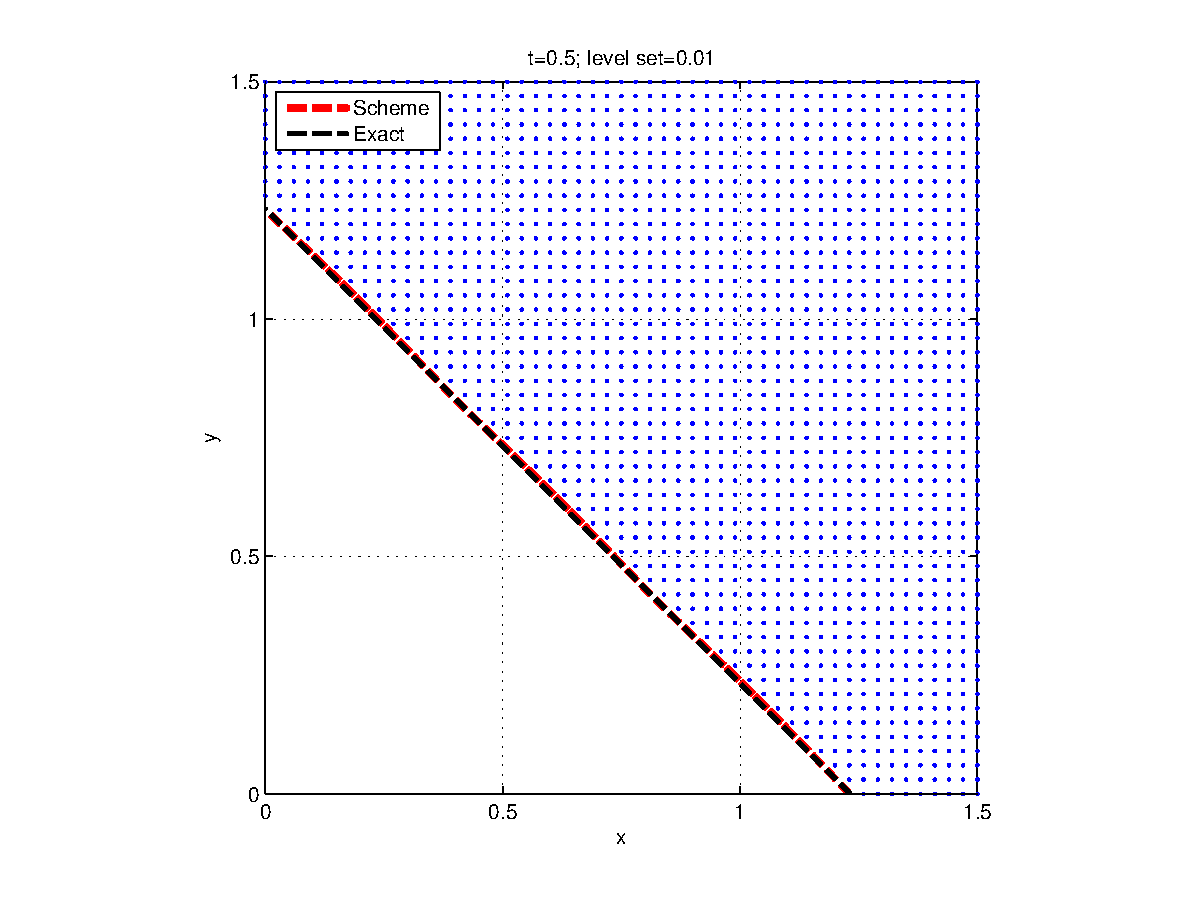
\includegraphics[scale=0.3]{EDP_isoline_lvlE-2.eps}
}
\caption[Payoff ]{Payoff \hspace{0.1cm}$ y=x_1+x_2$}
\label{fig: Results}
\end{figure}
\paragraph{Discretization error}
We have seen that the true error is linear in time discretization $h$ (conditionally to the fact that $\Delta x \approx h$. We can prove that by multiplying time step and spatial step by a same factor, called mesh scaling factor. The caculated errors should be approximately linear in this factor. 
\begin{table}[ht]
\centering 
\parbox{0.4\textwidth}{
\begin{tabular}{l|c|c|c}
ratio & $\mathbb{L}^{\infty}$ & $\mathbb{L}^{1}$ & $\mathbb{L}^{2}$  \\
\hline \hline
$2$    & 0.006000& 0.002108& 0.002600\\
$1.0$  & 0.003519& 0.000985& 0.001271\\
$2/3$  & 0.001798& 0.000601& 0.000753\\
$1/2$  & 0.001644& 0.000473& 0.000622\\
$1/3$  & 0.001170& 0.000311& 0.000406\\
$1/4$  & 0.000846& 0.000238& 0.000311\\
$1/5$  & 0.000860& 0.000191& 0.000250
\end{tabular}
}
\hspace{0.3cm}
\begin{minipage}[c]{0.53\textwidth}%
\hspace{0.5cm}
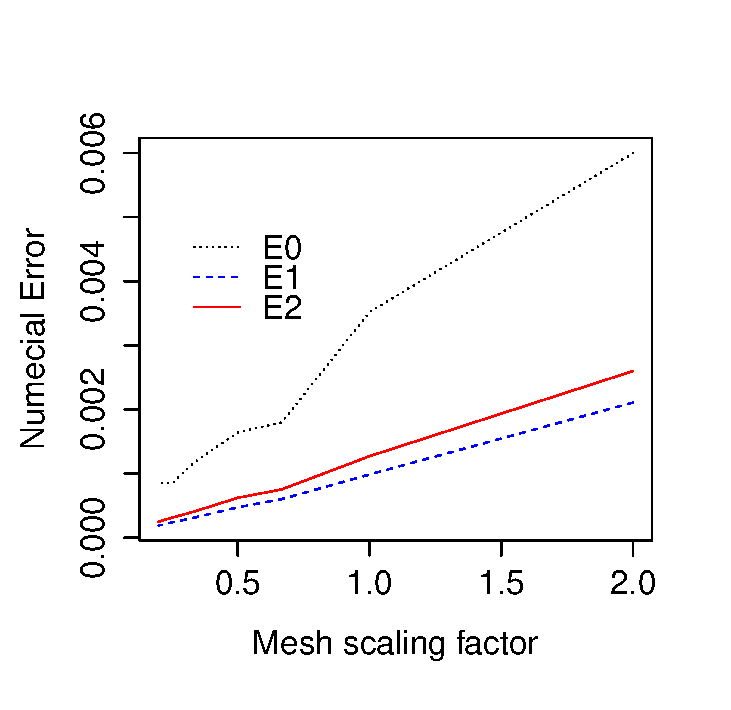
\includegraphics[scale=0.5,keepaspectratio=true]{linear_error}
\end{minipage}
\caption{Error linear in time step}
\label{table:error_linear}
\end{table}
As showed in the the \ref{table:error_linear}, the $\mathbb{L}^1$ seems the most stable amongs the 3 error types. Indeed the linearity is verified for $\mathbb{L}^1,\mathbb{L}^2$-norm.

\paragraph{Other payoff of basket option}
We also tried to turn our PDE with other basket payoff functions
\[
\varphi(S^1,S^2) = (K- \text{max}(S^1,S^2) )^+
\hspace{2cm}
\varphi(S^1,S^2) = (K- \text{min}(S^1,S^2) )^+
\]
the results from these payoff are as following :
\begin{figure}[ht]
\centering
\subfigure[$\varphi(S^1,S^2) = (K- \text{max}(S^1,S^2) )^+$]{
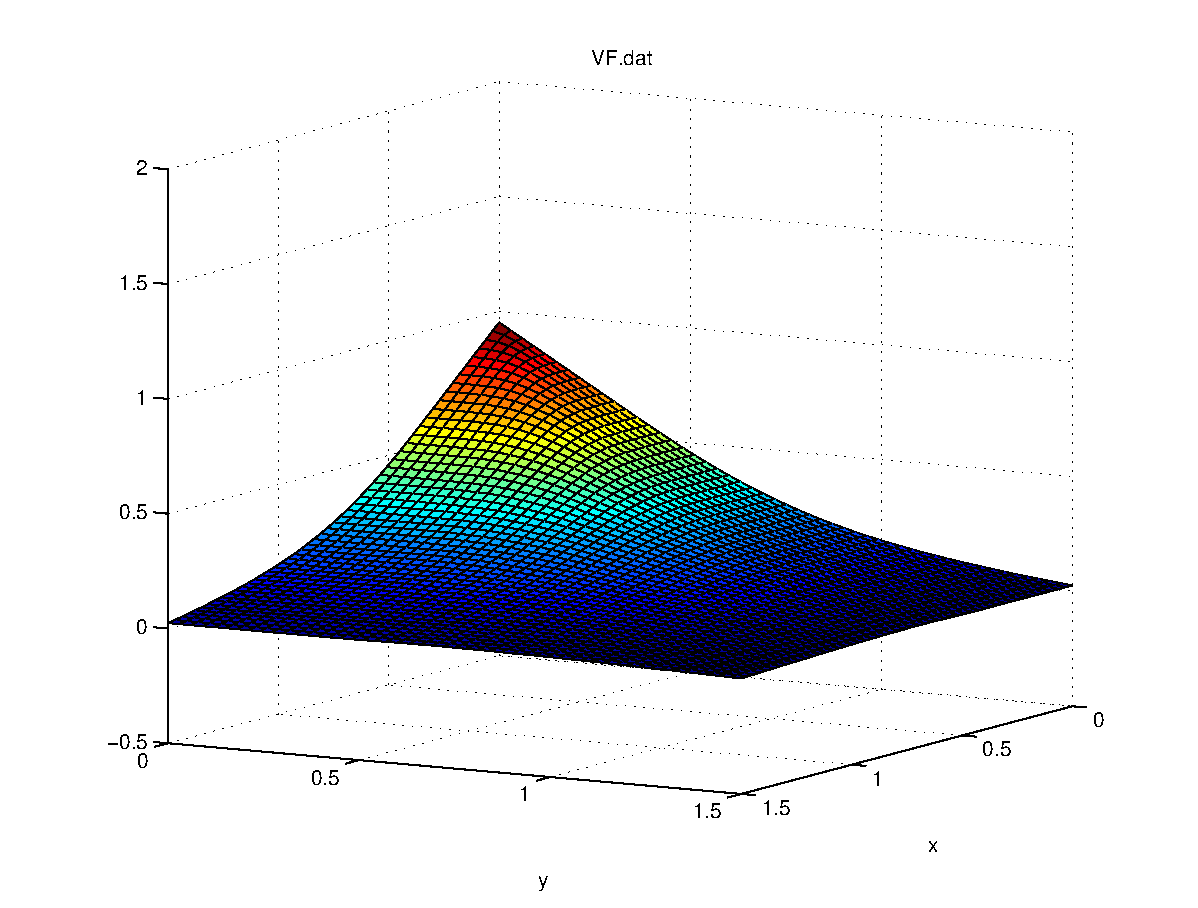
\includegraphics[scale=0.3]{put_max_2d.eps}
}
\quad
\subfigure[$\varphi(S^1,S^2) = (K- \text{min}(S^1,S^2) )^+$]{
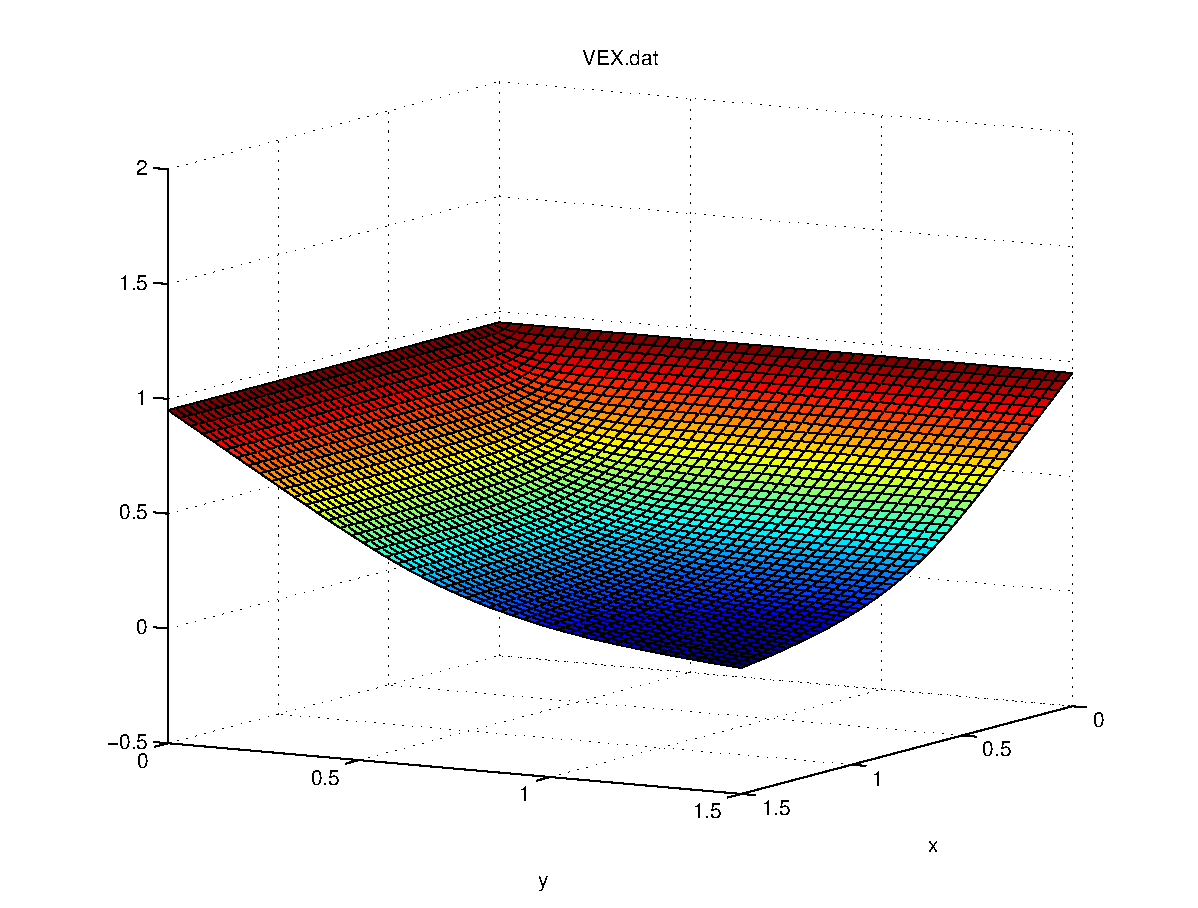
\includegraphics[scale=0.3]{put_min_2d.eps}
}
\caption[Payoff ]{Min-Max Payoff}
\label{fig:other_payoof}
\end{figure}


\subsection{Results in higher dimension}
We turned our PDE in higher dimension $d=1,2,3,4,5$in order to see the time required for each case.
\begin{center}
\begin{tabular}{l|c|c|c|c}
%%\hline
Dimension   &  2          & 3       & 4       & 5  \\
\hline\hline
Elapsed time(s)  &  0.00775807 & 0.10785 & 4.12525 & 182.404 \\
%\hline
\end{tabular}
\end{center}
For higher dimensional it is always possible to run the computation in condition to not precompute the grid's interpolation, but it required too much time. However, the algorithm, highly parrallelizable, is promising when it comes to very high dimensional issues.    
\section{Platen Scheme }
In this part we are going to discuss about the explicit scheme proposed by Platent. In particular, it involves the weak approximation of SDE's solution describing the underlying. \cite{Platen}ch15.1
\subsection{Scheme for d=1}
The idea is to approximate the SDE verified by S unidimensional by the following scheme
\begin{equation}
\begin{split}
Y_{n+1}=Y_n+&\frac{1}{2}(r\bar{\Upsilon}+rY_n)h+\frac{1}{4}(\beta\bar{\Upsilon}^+ + \beta\bar{\Upsilon}^-+2\beta Y_n)\Delta\hat{W}\\
&+\frac{1}{4}(\beta\bar{\Upsilon}^+ - \beta\bar{\Upsilon}^-)\left\lbrace(\Delta \hat{W})^2-h \right\rbrace h^{-1/2}\\
\end{split}
\end{equation}
where 
\begin{equation*}
\left\lbrace
\begin{array}{l}
\bar{\Upsilon}=Y_n + rY_nh + \beta Y_n \Delta \hat{W}, \\
\bar{\Upsilon}^{\pm}=Y_n + rY_nh \pm \beta Y_n \sqrt{h}
\end{array}
\right.
\end{equation*}
$\Delta\hat{W}$ could be Gaussian or it could be three points distributed with :
\begin{equation}
\mathbb{P}(\Delta\hat{W}=\pm \sqrt{3h})=\frac{1}{6} \hspace{2cm} \mathbb{P}(\Delta\hat{W}=0)=\frac{2}{3} 
\end{equation}
Let us befin three points following :
\begin{equation}
\begin{split}
\mathbb{E}[Y_{n+1}|Y_n=x]=\frac{2}{3} Y^{(0)}(x) +\frac{1}{6}Y^{(1)}(x) +\frac{1}{6}Y^{(-1)}(x) 
\end{split}
\end{equation}
where (c.f. annexe \ref{Platen calculus})
\begin{equation}
\left\lbrace
\begin{array}{l}
Y^{(0)}(x)           =x+h[-\frac{\beta^2 x}{2}  +rx ] +\frac{h^2}{2}r^2x  \\ \\
Y^{(\varepsilon)}(x) =Y^{(0)}(x)  + \frac{3}{2}\beta^2xh +\varepsilon\sqrt{3}\beta x (h^{1/2}+h^{3/2}r),  \hspace{1cm}  \varepsilon \in \{-1;1\}
\end{array}
\right.
\end{equation}
The semi-Lagrangian version of Platen scheme will be : 
\begin{equation}
u_n(x) = \frac{e^{-rh}}{3}\left\lbrace2u_{n+1}(Y^{(0)}(x))+ \frac{u_{n+1}(Y^{+}(x))}{2}+ \frac{u_{n+1}(Y^{-}(x))}{2}\right\rbrace
\end{equation}
\subsection{Multidimesional scheme}
In this section, we propose two approachs for high dimension resolution via Platen scheme. The first one comes directly from the one dimensional scheme whereas the second one involves the mutltidimensional Platen scheme which is much more sophisticated.
\subsubsection{Generalization from unidimensional scheme}
The first idea is to approximate each direction, equally probably, of diffusion $\sigma_k(x)=x*\beta_k$. Given that each direction is equally probably, we just need to uniformly normalize for $d$-dimentional increment $\Delta \hat{W} \in \mathbb{R}^d$
\begin{equation}
u_n(x) = \frac{e^{-rh}}{6d}\sum^d_{k=1} \left\lbrace u_{n+1}[Y^{j-}_k(x)] +  4u_{n+1}[Y^{(0)}_k(x)]+ u_{n+1}[Y^{j+}_k(x)] \right\rbrace
\end{equation}
where \footnote{We define the $*$ operator as $[a*b*c]_i = a_ib_ic_i$}

\begin{equation}
\left\{
\begin{array}{ll}
Y^{(0)}_k(x)           =& x+h\left\lbrack-\frac{x*\beta_k*\beta_k}{2}+rx\right\rbrack + \frac{h^2}{2}r^2 x \\
Y^{(\varepsilon)}_k(x) =& Y^{(0)}_k(x)+h\frac{3d}{2}(x*\beta_k*\beta_k)+\varepsilon\sqrt{3d} \left( rh^{3/2}+h^{1/2} \right)x*\beta_k 
\end{array}
\right.
\end{equation}
\paragraph{Implemented scheme}
We turn a loop over $k,\varepsilon$
\begin{equation}
Y_{k,\varepsilon}(x) = x 
                     + (h + \frac{h^2r}{2}  ) rx
                     + \varepsilon \sqrt{3dh}(rh + 1 )  x*\beta_k
                     + \frac{h}{2}(-1 + \varepsilon^2 3d)x*\beta_k*\beta_k                     
\end{equation}
We have tested this scheme and compared to the Euler first order scheme. The results is not better. Maybe, some adjustement of required points need to be carried out.
\begin{figure}[ht]
\centering
\subfigure[$\varphi(S^1,S^2) = (K- \text{max}(S^1,S^2) )^+$]{
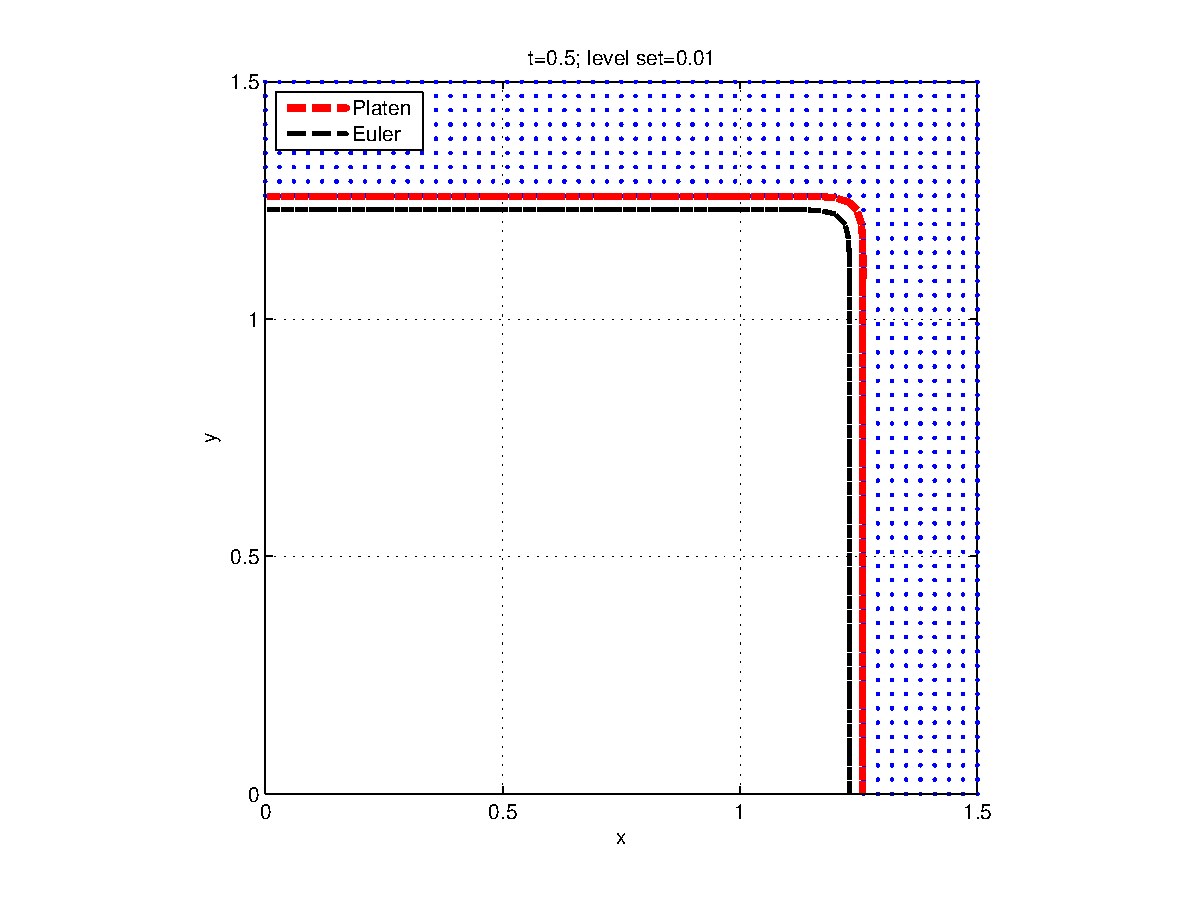
\includegraphics[scale=0.3]{put_max_vs.eps}
}
\quad
\subfigure[$\varphi(S^1,S^2) = (K- (S^1+S^2) )^+$]{
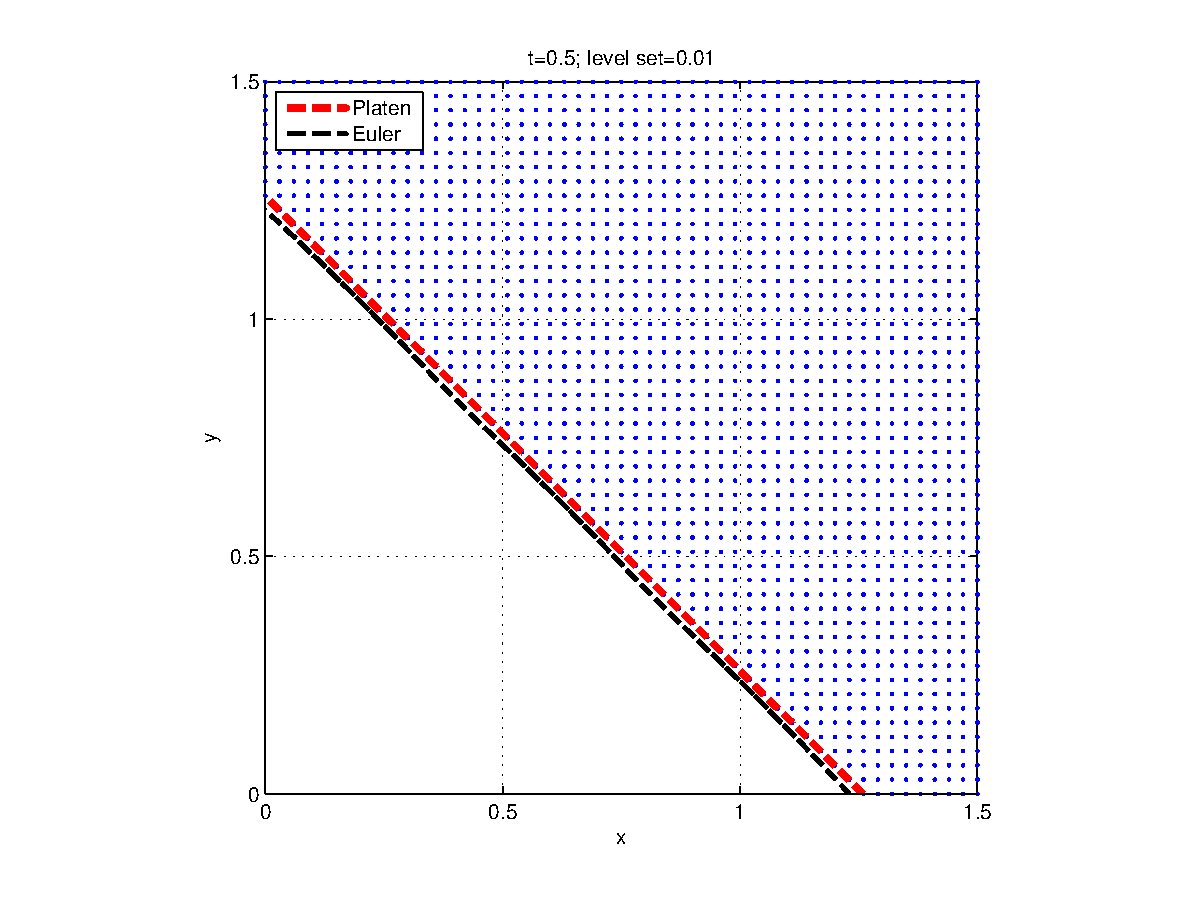
\includegraphics[scale=0.3]{put_weighted_vs.eps}
}
\caption[Payoff ]{Platen vs. Euler result}
\label{fig:other_payoof}
\end{figure}
\subsubsection{Multidimesional Platen Scheme}
We give here the multidimentional counterpart of the Platen unidimensional scheme. The vector form of multidimentional approximation is 
\begin{equation}
\begin{split}
  &Y_{n+1} = Y_{n} + 
	  \underbrace{\frac{1}{2}( r\bar{\Upsilon}  + rY_n)h}_{\textbf{I}(Y_n)} \\
         &+\sum^d_{j=1}\underbrace{\frac{1}{4}  \left\{
                           \left[  \sigma_j(\bar{R}^j_+ )  +  \sigma_j(\bar{R}^j_- )  + 2\sigma_j(Y_n)  \right]\Delta \hat{W}^j 
         +\sum^d_{r\neq j} \left[  \sigma_j(\bar{U}^r_+ )  +  \sigma_j(\bar{U}^r_- )  - 2\sigma_j(Y_n)  \right]\Delta \hat{W}^j 
                       \right\}}_{\textbf{II}_j(Y_n)}  \\
	  &+\sum^d_{j=1}\underbrace{\frac{1}{4\sqrt{h} }\left\{
			    \left[  \sigma_j(\bar{R}^j_+ )  -  \sigma_j(\bar{R}^j_- )  \right] \left\{ (\Delta \hat{W}^j)^2 - h \right\}
         +\sum^d_{r\neq j} \left[  \sigma_j(\bar{U}^r_+ )  -  \sigma_j(\bar{U}^r_- )  \right] \left\{ \Delta\hat{W}^r\Delta\hat{W}^j + V_{r,j} \right\}
                       \right\}}_{\textbf{III}_j(Y_n)}
\end{split}
\end{equation}
Where \footnote{The drift term is $r[x]$ and the diffusion term is $\sigma_j(x)=\textbf{diag}(x)\beta^j$}
\begin{equation*}
\left\lbrace
\begin{array}{l}
\bar{\Upsilon}=Y_n + rY_nh + \sum^d_{j=1} \sigma_j(Y_n) \Delta \hat{W}^j, \\ \\
\bar{R}^j_{\pm}=Y_n + rY_nh \pm \sigma_j (Y_n) \sqrt{h}, \\ \\
\bar{U}^j_{\pm}=Y_n  \pm \sigma_j (Y_n) \sqrt{h}
\end{array}
\right. \hspace{1cm}
\left\lbrace
\begin{array}{l}
\Delta \hat{W}^j \in \left\{ (-\sqrt{3h},\frac{1}{6}),(0,\frac{2}{3}),(\sqrt{3h},\frac{1}{6})   \right\} \\ \\
V_{r,j} \in  \left\{ (-h,\frac{1}{2}),(h,\frac{1}{2}))   \right\}, \hspace{0.5cm} r < j \\
V_{j,j} = -h \\
V_{r,j} = -V_{j,r} , \hspace{2.5cm} r > j
\end{array}
\right. 
\end{equation*}
We have : 
\begin{equation*}
\begin{split}
\textbf{I}(x)   %& = \frac{1}{2} \left[ r\left(x+rhx+ \sum^d_{j=1} \textbf{diag}(x)\beta^j \Delta\hat{W}^j\right)  + rx  \right] h \\ 
                & = \frac{1}{2} \left[ 2rx  + r \sum x*\beta_j \Delta\hat{W}^j  + hr^2x \right] h \\ \\
\textbf{II}_j(x)  & = \frac{(2+rh)}{2} x*\beta_j \Delta \hat{W}^j \\ \\
\textbf{III}_j(x) & =  \sum^d_{r=1} \underbrace{\frac{1}{2}<\beta_r,\beta_j>  \left[ \Delta \hat{W}^r \Delta \hat{W}^j + V_{r,j} \right] x}_{\textbf{III}_{r,j}(x)}
\end{split}
\end{equation*}
Due to the limited time, we didn't succeed in implementing this scheme.  

\section{Conclusion}
In this project, we have studied the PDE's pricing for mutltidimensional Black Scholes. Generally, a closed form solution doesn't exist  except for some particular payoff. We have exposed three schemes for numerical solution. All of them are based on martigale property of the underlying and the approximation of SDE via Markov chains. The first order approximation via Markov chains gives the Euler approximation thus its Semi-Lagragian version of PDE's pricing. We have succeeded in proving the consistency of first order scheme by numerical results. We have used the multidimensional PDE solver \textbf{ROC-HJ solver}\cite{BokanowskiLib}. As for the second order approximation, we have proposed two approachs. We have implemented the first one but haven't succeeded in proving the second order convergence due to the simplicity of the scheme. Only the theoretical part of second proposal, apparently more accurate but deman ding more time to implement, was exposed in this report.  

\section{Annex}
\subsection{Proof of lemma}
\begin{lemma*}
Let $v:[0,T]\mathbb{R}^d \longrightarrow \mathbb{R} $ a sufficiently regular function. We have :
\begin{align*}
\sum_{\varepsilon={-1,1}}v(t,x+\varepsilon\sqrt{h}y)
& = 2v(t,x) + h\sum_{i,j=1}^d y_{i}y_{j}\partial^2_{ij}v(t,x) + O(h^2.||\textbf{D}^4_xv||_\infty)\\
& = 2v(t,x) +  O(h.||\textbf{D}^2_xv||_\infty)
\end{align*}
\end{lemma*}
\begin{proof}
Indeed, we write Taylor formula between $x + \varepsilon\sqrt{h}y$ and $x$ : 
\begin{align*}
\sum_{\varepsilon={-1,1}}v(t,x + \varepsilon\sqrt{h}y) 
=&\sum_{\varepsilon={-1,1}} [ v(t,x) + \varepsilon \sqrt{h} \sum_{i=1}^d  y_{i}\partial_i v(t,x) \\
 &+\frac{h}{2} \sum_{i,j=1}^d y_{i}y_{j}\partial^2_{ij}v(t,x) 
  +\varepsilon^3 \frac{h\sqrt{h}}{6} \sum_{i,j,l=1}^d y_{i}y_{j}\bar{\sigma}_{kl}\partial^3_{ijl}v(t,x) \\
 &+\frac{h^2}{24}\sum_{i,j,l,m=1}^d y_{i}y_{j}y_{l}y_{m}\partial^4_{ijlm}v(t,x)] 
  + o(h^2)\\
 =\hspace{0.1cm}& 2v(t,x) + h\sum_{i,j=1}^d y_{i}y_{j}\partial^2_{ij}v(t,x) + O(h^2.||\textbf{D}^4_xv||_\infty) \qed
\end{align*}
\end{proof}
\subsection{Platen scheme} \label{Platen calculus}
Calculus example for $Y^{(0)}$
\begin{equation}
\begin{split}
Y^{(0)}(x) &=x+\frac{1}{2}(r(x+rxh)+rx)h  
		-\frac{1}{4}(\underbrace{\beta(x+rxh+\beta x \sqrt{h})-\beta(x+rxh-\beta x \sqrt{h})}_{2\beta^2 x \sqrt{h}})\sqrt{h}\\
		&=x+h[(-\frac{\beta^2 x}{2}  +rx ] +\frac{h^2}{2}r^2x
\end{split}
\end{equation}


\bibliographystyle{siam}
\bibliography{EDPPhi}
\end{document}
